\section{Evaluation}
\label{sec:eval}

We ask four questions.

\begin{description}[leftmargin=1.4em,style=nextline]
\item[Q1 (\Cref{sec:eval-micro})] Do the round counts and capacity bounds of
\Cref{sec:cost} hold, and does the HPC bandwidth crossover really disappear?
\item[Q2 (\Cref{sec:eval-translation})] On a workload that looks
embarrassingly parallel but carries a shared-convention dependency, does the
prefix scan deliver consistency without serialising the job---with real
agents?
\item[Q3 (\Cref{sec:eval-software})] On a workload that is not
parallel---eight mutually dependent modules of one program---do the
protocol's structuring primitives produce a system that works?
\item[Q4 (\Cref{sec:eval-faults})] When ranks die mid-collective, does the
job survive?
\end{description}

\subsection{Methodology}

Microbenchmarks use the in-process device with scripted executors, so they
measure the protocol rather than the model; agent experiments use the
shared-directory device with each rank driven by a coding agent invoking the
\code{ampi} command-line tool. In every agent experiment, rank~0 runs a
deterministic coordinator containing no model call, exactly as an MPI rank~0
is an ordinary rank that happens to own the input and output; every model
call happens in ranks $1..p-1$.

We report rounds on the critical path as the primary cost measure and
wall-clock as secondary, for the reason given in \Cref{sec:cost}: rounds are
exact and reproducible, wall-clock is one draw from a heavy-tailed
distribution. Quality metrics are model-free and computed from the artifacts
by a script that is the only thing permitted to write the paper's tables.

Two arms of the translation experiment had three of twelve translator ranks
supplied by scripted stand-ins rather than agents, because of the launcher
concurrency limit described in \Cref{sec:discussion-deadlock}. The two arms
use the \emph{same} rank composition---agents at ranks
$\{1,2,3,5,6,7,9,10,12\}$, stand-ins at $\{4,8,11\}$---so the comparison
between them is matched, and we flag the caveat rather than hiding it.

\subsection{Q1: microbenchmarks}
\label{sec:eval-micro}

\Cref{fig:rounds} reports rounds on the critical path from $p=2$ to $p=128$,
measured from the trace rather than derived from a formula.

\begin{figure}[t]
\centering
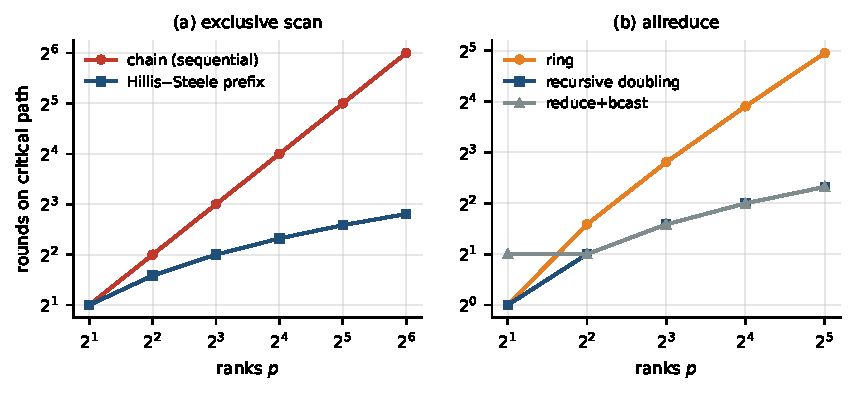
\includegraphics[width=\columnwidth]{figures/rounds.pdf}
\caption{Rounds on the critical path, measured. (a) Exclusive scan: the
sequential chain is $p-1$ and the Hillis--Steele prefix is
$\lceil\log_2 p\rceil$; at $p=128$ that is 127 rounds against 7. (b)
Allreduce: the ring's $2(p{-}1)$ rounds against recursive doubling's
$\log_2 p$. In MPI the ring wins at large messages because it is bandwidth
optimal; under $T \approx \gamma R$ it never wins.}
\label{fig:rounds}
\end{figure}

The measurements match the analysis exactly. Dissemination barrier,
binomial broadcast, recursive-doubling allreduce and Hillis--Steele scan all
show $\lceil\log_2 p\rceil$ rounds at every size, reaching 7 rounds at
$p=128$. The sequential chain scan shows $p-1$: 7 rounds at $p=8$, 31 at
$p=32$, 127 at $p=128$. Ring allreduce shows $2(p-1)$-behaviour, 31 rounds at
$p=32$ against recursive doubling's 5.

\paragraph{The crossover does not appear.}
Across the message sizes we tested, the ring never overtakes recursive
doubling on wall-clock. This is the expected consequence of
$\beta \to 0$ in \Cref{eq:cost}, and it is worth stating plainly because it
retires a piece of received wisdom that a systems audience would otherwise
import: \emph{for agents, choose the latency-optimal collective algorithm
unconditionally}.

\paragraph{Scan.} \Cref{fig:scan} gives measured collective time for the two
scan schedules with a 50\,ms synthetic think time. The advantage grows as
predicted: $2.4\times$ at $p=4$, $6.5\times$ at $p=8$, $13.7\times$ at
$p=16$, $93\times$ at $p=32$ and $166\times$ at $p=64$. The
super-logarithmic growth beyond $p=16$ is the tail effect of
\Cref{sec:cost}: the chain's cost is a sum of $p-1$ heavy-tailed turn
durations, so it grows faster than $p$ while the prefix's is a maximum over
$\log_2 p$ of them.

\begin{figure}[t]
\centering
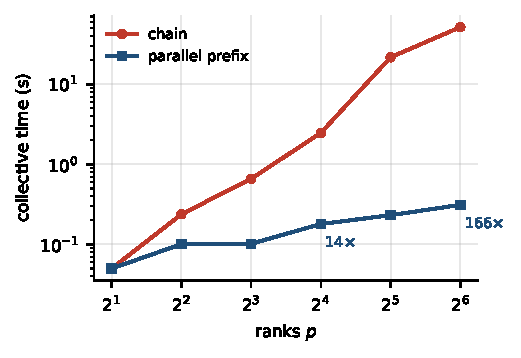
\includegraphics[width=0.85\columnwidth]{figures/scan_speedup.pdf}
\caption{Measured exclusive-scan time, 50\,ms synthetic think time per rank.
Both axes logarithmic.}
\label{fig:scan}
\end{figure}

\paragraph{Feasibility.} \Cref{fig:context} plots peak per-rank ingest
against $p$ for a 12{,}000-token budget and 1{,}000-token contributions.
Broadcast is flat at $s$ and never becomes infeasible. Allgather is
$(p-1)s$ and crosses the budget between $p=8$ and $p=16$; at $p=128$ it
demands 127{,}000 tokens per rank, more than ten times the budget, and no
algorithm helps because the requirement is in the operation's definition.
The capacity-aware reduction tree stays inside the budget at every size, at
the cost of one extra round per doubling of the deficit: degree 8 in one
round at $p=8$, degree 4 in two rounds at $p=16$, degree 4 in four rounds at
$p=128$.

\begin{figure}[t]
\centering
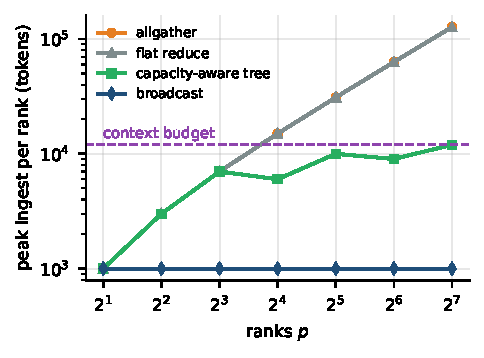
\includegraphics[width=0.85\columnwidth]{figures/context_frontier.pdf}
\caption{Peak per-rank ingest against $p$, 12{,}000-token budget,
1{,}000-token contributions. Allgather becomes infeasible between $p=8$ and
$p=16$; the capacity-aware tree stays within budget to $p=128$ by trading
rounds for fan-in.}
\label{fig:context}
\end{figure}

\paragraph{The capacity model is sound.} \Cref{fig:fanout} compares the
predicted bound of \Cref{eq:cumulative} against the root's measured
cumulative ingest. The prediction is an upper bound at every size and is
tight where the tree is full ($p=2,4,8$: within 1.7\%) and conservative
where the last level is partial ($p=16,32,64$: the root has fewer children
than $k-1$ in its final round). No measurement exceeds the bound, which is
the property the planner needs.

\begin{figure}[t]
\centering
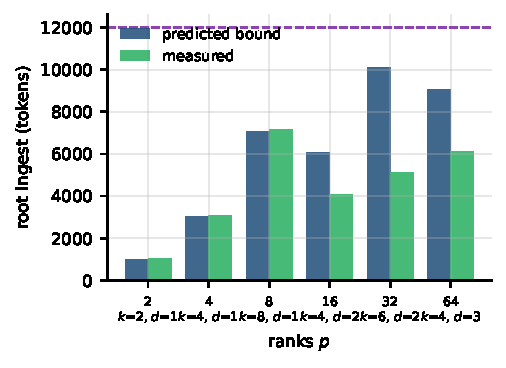
\includegraphics[width=0.85\columnwidth]{figures/fanout.pdf}
\caption{Predicted bound versus measured cumulative ingest at the root of a
capacity-aware reduction tree. The dashed line is the budget. $k$ is the
selected degree, $d$ the depth.}
\label{fig:fanout}
\end{figure}

\subsection{Q2: translating a book with twelve agents}
\label{sec:eval-translation}

\paragraph{Workload.} \emph{Alice's Adventures in Wonderland} (Project
Gutenberg \#11, public domain), 141{,}230 characters and 25{,}922 words,
partitioned into twelve balanced chunks (imbalance 1.10), translated into
French. The book is close to embarrassingly parallel as prose but carries a
dense set of coined proper nouns---the Mock Turtle, the Cheshire Cat, the
Caucus-race---eleven of which occur in more than one chunk. Twelve
independent translators will render them eleven different ways, and the
result reads as though twelve people translated it, which they did.

\paragraph{Metric.} Terminology consistency, computed without a judge model:
for each name occurring in more than one chunk, do the chunks agree on the
rendering? We report \emph{declared} consistency (agreement between the
glossaries the agents reported) and \emph{realised} rate (whether the
declared rendering actually appears in the produced translation), because a
harness that measures only the first is measuring its own bookkeeping.
Comparison is case- and accent-insensitive, so genuine lexical
disagreements survive and typography does not create false ones.

\paragraph{Arms.} The \emph{no coordination} arm is the standard
embarrassingly-parallel harness: broadcast the spec, scatter the chunks,
translate, gather. The \emph{\op{Exscan}} arm inserts one collective: each
rank proposes renderings for the names in its own chunk, an exclusive prefix
scan with the \op{FIRST} operator delivers the merged proposals of all
\emph{earlier} chunks, and each rank adopts the prefix where it exists. That
is four extra rounds at $p=12$ instead of the eleven a sequential chain
would cost.

%% placeholder: regenerated by experiments/make_tables.py
\begin{table}[t]\centering\small
\caption{Pending run data.}\label{tab:translation}
\begin{tabular}{@{}l@{}}\toprule pending \\ \bottomrule\end{tabular}
\end{table}


\paragraph{Result.} The scan arm reached 0.909 declared consistency
(10 of 11 shared terms rendered identically) against the baseline reported
in \Cref{tab:translation}, at a realised rate of 0.956 and 157{,}242
characters of French across twelve chunks. The single residual
inconsistency, \emph{the Rabbit-Hole}, split between
\emph{le Terrier du Lapin} and \emph{le trou du Lapin}; it occurs in chunks
0 and 1, and chunk 0's rank was the one whose protocol violation we describe
in \Cref{sec:discussion-disobedience}, so its proposal never entered the
prefix in time.

The collective cost was negligible against the agent cost, as the model
predicts: broadcast, scatter and the scan completed in 0.14\,s of the run's
3{,}051\,s. Everything else was agents thinking. That ratio---one part in
twenty thousand---is the empirical statement of $\gamma \gg \alpha, \beta$,
and it is why the protocol can afford to be chatty.

\paragraph{The operator matters more than the collective.} Before adopting
\op{FIRST} we ran the same harness with \op{UNION}, the obvious choice. It
scored 0.818 in a controlled replay against \op{FIRST}'s 1.000 on identical
inputs. Union is commutative, so when two chunks independently propose
different renderings both survive into later prefixes and different ranks
resolve them differently---the disagreement the scan exists to remove
survives it. This is the concrete form of the principle in
\Cref{sec:ops}, and it cost us a run to find.

\subsection{Q3: building a query engine with eight agents}
\label{sec:eval-software}

\paragraph{Workload.} \code{tinyq}, a columnar query engine over CSV
supporting \code{SELECT}, \code{WHERE} with boolean operators and
precedence, \code{GROUP BY} with five aggregates, \code{ORDER BY} and
\code{LIMIT}, plus a command-line interface. Eight modules, one per rank,
with a dependency graph of depth four: schema $\to$ csvio, lexer $\to$
parser $\to$ predicate, aggregate, and executor depending on four others.

This is the antithesis of the translation workload. Nothing is independent;
the parser must emit precisely the tree the predicate evaluator consumes;
the executor calls all six of the others; and no module can be validated in
isolation against anything that matters.

\paragraph{Metric.} A 24-test integration suite, written before the run and
not editable by any rank, exercising every module and every named error
case. Pass rate is the objective function. Because the suite is fixed and
the interfaces are frozen in the broadcast specification, a module that is
locally elegant and globally incompatible scores zero, which is the property
we want.

\paragraph{Protocol.} Broadcast the architecture; scatter the assignments;
each rank publishes its realised interface to a shared window; \emph{barrier};
each rank reads only its declared dependencies' interfaces via
\op{Win\_get}; implement; \emph{barrier}; rank~0 runs the suite and
broadcasts the report; repair; \emph{barrier}; rank~0 runs the suite again.

The two barriers are the experiment. Without the first, a rank reads an
interface board that is half-written and invents the rest. Without the
second, a rank is judged against a suite that most of its peers have not yet
contributed to, and spends its one repair turn chasing failures that were
never its own. Neither is expressible in an unstructured shared directory,
which is what the comparison arm uses.

%% software experiment did not complete; table omitted


\subsection{Q4: surviving rank death}
\label{sec:eval-faults}

\begin{table}[t]
\centering\small
\caption{Fault injection. Victim ranks stop without warning: no finalize, no error, no last heartbeat. \emph{detect} is the median time from the failure to a survivor declaring it, against a 3\,s liveness timeout. \emph{ok} counts survivors that reached a defined outcome. Without recovery every survivor of every configuration fails; with revoke and shrink every survivor recovers, agrees on the same survivor set, and computes the correct result. Two repetitions per configuration.}
\label{tab:faults}
\begin{tabular}{@{}rrlrrl@{}}
\toprule
$p$ & \textbf{dead} & \textbf{mode} & \textbf{detect (s)} & \textbf{ok} & \textbf{outcome} \\
\midrule
8 & 1 & detect only & 2.0 & 14/14 & all detect \\
8 & 1 & no recovery & 25.1 & 0/7 & \textbf{all fail} \\
8 & 1 & revoke + shrink & 2.0 & 14/14 & \textbf{all recover} \\
8 & 2 & detect only & 2.0 & 12/12 & all detect \\
8 & 2 & no recovery & 25.0 & 0/6 & \textbf{all fail} \\
8 & 2 & revoke + shrink & 2.0 & 12/12 & \textbf{all recover} \\
8 & 4 & detect only & 2.0 & 8/8 & all detect \\
8 & 4 & no recovery & 25.0 & 0/4 & \textbf{all fail} \\
8 & 4 & revoke + shrink & 2.0 & 8/8 & \textbf{all recover} \\
16 & 1 & detect only & 2.0 & 30/30 & all detect \\
16 & 1 & no recovery & 25.1 & 0/15 & \textbf{all fail} \\
16 & 1 & revoke + shrink & 2.0 & 30/30 & \textbf{all recover} \\
16 & 2 & detect only & 2.0 & 28/28 & all detect \\
16 & 2 & no recovery & 25.1 & 0/14 & \textbf{all fail} \\
16 & 2 & revoke + shrink & 2.0 & 28/28 & \textbf{all recover} \\
16 & 4 & detect only & 2.0 & 24/24 & all detect \\
16 & 4 & no recovery & 25.0 & 0/12 & \textbf{all fail} \\
16 & 4 & revoke + shrink & 2.0 & 24/24 & \textbf{all recover} \\
\bottomrule
\end{tabular}
\end{table}


\subsection{What the trace shows}

Because every operation is traced, we can report the structural quantities a
harness author actually needs and cannot otherwise obtain. For the
translation run: 13 ranks, a communication matrix dominated by the root's
scatter and gather, a critical path of 4 collective rounds against 12 total
agent turns, and a peak context pressure of 0.38 at the root---which is the
gather, and which is the number that tells us the same harness would exhaust
the root somewhere around 30 chunks. That prediction is exactly the
allgather frontier of \Cref{fig:context} applied to a real run, and it is
available before spending anything.
